\chapter{Design and implementation}
\label{chap:design}

\section{Design principles and architecture}

The central design problem is separating planning from permission. A browser
agent needs enough freedom to interpret a page, recover from errors, and choose
its next step. Yet the model that proposes that step should not also decide
whether it is safe to execute. \systemname\ therefore leaves planning to
BrowserUse and independently governs both the information that reaches the
planner and the effects that reach the privileged executor. Four principles
turn that separation into a runtime architecture.

\begin{enumerate}
  \item \textbf{Keep authority outside the acting model.} The model receives
  observations and tool outcomes, but only the middleware can reach the
  privileged executor.

  \item \textbf{Mediate both sides of the agent loop.} The observation guard
  reduces known hostile influence before inference. The action guard then
  constrains the resulting effect, including when hostile influence or an
  ordinary planning error survives.

  \item \textbf{Represent consent as bounded authority.} Approval is tied to
  reviewed live context and checked again before execution. Protected input is
  withheld from the agent and entered directly by the operator.

  \item \textbf{Fail closed and retain accountable outcomes.} Missing context,
  unresolved sanitisation, silence, timeout, stop, or malformed authority
  cannot become permission. Decisions remain inspectable without reproducing
  the sensitive content that caused them.
\end{enumerate}

Together, these principles preserve planning flexibility while making
permission a system property. BrowserUse plans and recovers from ordinary
errors; Sentinel owns the guards, authority, and audit that govern each effect,
as \cref{fig:architecture} shows.

\begin{figure}[!t]
\centering
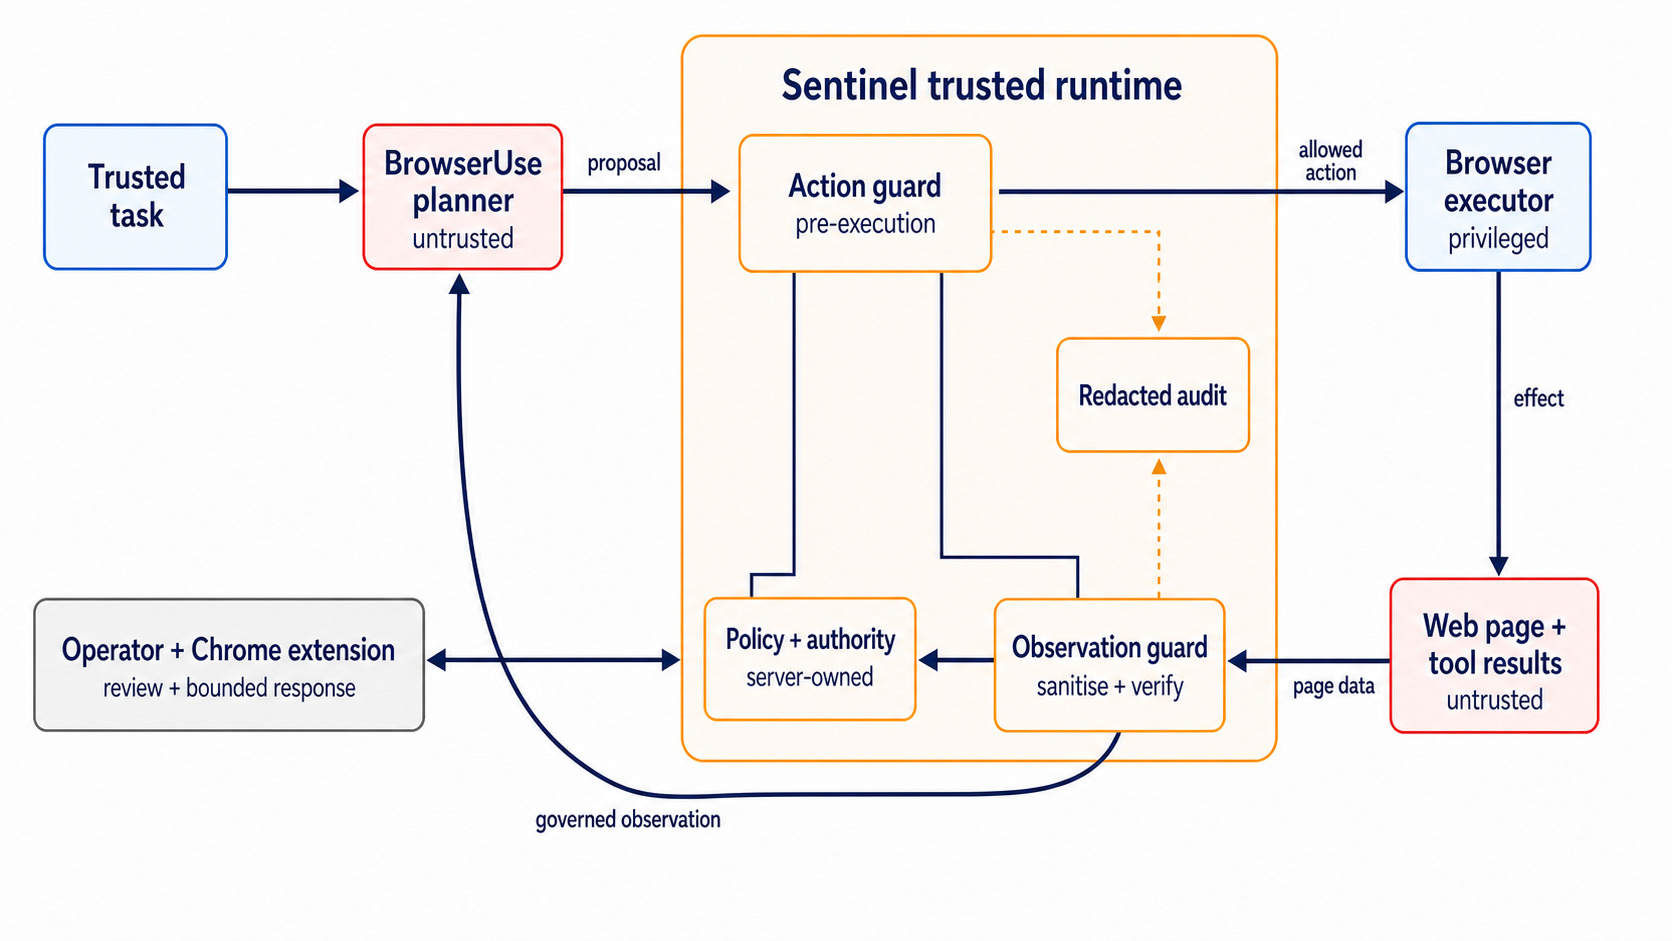
\includegraphics[width=\textwidth]{figures/sentinel-runtime-architecture-v2.png}
\caption{Sentinel's two runtime guards and server-owned authority flow.}
\label{fig:architecture}
\end{figure}
\FloatBarrier

Read from left to right, a trusted task reaches the planner, whose proposal
crosses the action guard before the executor may change the browser. The return
path carries page and tool data through the observation guard before a governed
representation reaches the planner. Policy and authority inform both guards,
while audit records each outcome.

The chapter first follows this governed runtime path through observation,
action, authority, and audit. It then turns to the Chrome extension, which
projects the resulting server-owned state into the browser without becoming a
second source of permission.

\section{Runtime architecture}

\subsection{Composition and supported channel}

Sentinel runs as a Python service around an ordinary BrowserUse agent, without
forking BrowserUse. A model wrapper governs the planner's observations, while a
tool wrapper mediates each proposed effect immediately before execution. These
components, \texttt{GovernedLLM} and \texttt{GovernedTools}, retain BrowserUse's
normal interfaces~\cite{zunic2026browseruse}.

Each task receives run-local budgets, findings, grants, interventions, latency,
cancellation state, and a fresh key for HMAC digests. This boundary prevents
authority and linkable audit evidence from carrying into a later task.

The model-input channel is deliberately textual. Sentinel removes images from
current-state and tool-result messages, discards remaining frame captures,
wraps browser-derived text as untrusted, and reduces sensitive URL metadata.
The evaluated planner therefore receives a DOM/accessibility representation
that Sentinel can inspect and rewrite. Pixel-only instructions and visually
grounded tasks fall outside this channel. A multimodal planner would need a
separate visual-observation guard.

Sentinel exposes three runtime modes, distinguished by whether security
decisions are evaluated and enforced. Off skips prompt-injection detection and
makes the action policy return allow, although redacted action attempts and
terminal outcomes are still audited. Shadow runs the detector and action-policy
rules against live context, but neither rewrites the checked model input nor
applies a policy-derived verdict. Instead, it records the detections and the
block, approval, or handoff that would have occurred. Enforce applies those
outcomes: it may sanitise or withhold a detected observation; for an action
proposal, it may allow, block, request approval, or require a human step. In the
evaluation, \emph{full} denotes enforce mode with both guards enabled; it is an
experimental condition, not a fourth runtime mode. Across every mode, the
supported model channel remains text-only, tool results remain marked as
untrusted, and navigation metadata remains redacted.

Sentinel checks cancellation around every authority wait and immediately before
execution. Approval and human-control deadlines expire before the outer step
timeout, so denial, timeout, cancellation, and shutdown close the proposal.

\subsection{One governed agent step}

A BrowserUse step may return a short, ordered sequence of model-proposed
actions. Sentinel treats each action as a separate proposal with its own
authority decision and terminal outcome:

\begin{enumerate}[leftmargin=8mm]
  \item \textbf{Capture.} The observation wrapper separates the trusted task
  from DOM-derived state and bounded tool results, normalises them, and removes
  sensitive URL metadata.

  \item \textbf{Sanitise and verify.} Enforce mode rewrites attributable
  findings, reconstructs the provider message, and scans it again. If that
  message is not detector-clear, Sentinel withholds it before the model request.

  \item \textbf{Plan.} The model receives the governed representation and
  returns BrowserUse proposals with no authority to produce their intended
  effects.

  \item \textbf{Rebuild authority.} For each proposal, the action wrapper
  records the attempt and reconstructs live origin, target, policy, destination,
  protected-data class, and taint. Policy allows, blocks, requests approval, or
  requires handoff. Approval triggers complete preflight again; handoff
  withholds the proposal for direct operator action.

  \item \textbf{Execute and close.} Only an allowed, still-valid proposal
  reaches the tool. Its audit pair closes before the next proposal; an error,
  sequence-terminating action, or URL or focus change abandons the remainder.
\end{enumerate}

Observation governance comes first: a later block cannot undo a plan already
shaped by hostile content. Even so, action governance repeats for every
proposal, since page, target, and policy state can change after planning.

\section{Observation governance}
\label{sec:observation-governance}

\subsection{Untrusted regions and representation boundaries}

Sentinel separates trusted task context from browser state, page extractions,
and tool results, scanning only these untrusted regions. It also escapes
reserved protocol tags inside textual tool results before wrapping them as
untrusted history.

If a page imitates BrowserUse or Sentinel prompt structure, \emph{boundary
neutralisation} escapes reserved tags only inside a recognised untrusted
region. Genuine outer wrappers and ordinary DOM tags remain unchanged, so
forged syntax cannot create a trusted region or close the real one.

Model-facing browser state also withholds titles and replaces each HTTP(S)
query string and fragment wholesale. For \texttt{data:}, \texttt{javascript:},
\texttt{blob:}, \texttt{file:}, and other non-web URLs, only the scheme is
retained in model input, runtime events, and persistent traces. The opaque
suffix may contain a document, script, path, or identifier. General telemetry
retains safe HTTP(S) context while redacting recognised sensitive values.

\subsection{Detection and attributable sanitisation}

The detector scores instruction override, authority impersonation, role
reassignment, evasion, exfiltration, forged markup, and encoded instructions.
One strong signal can cross the threshold; weaker cues must combine. The source
origin then remains tainted for the run, since earlier content may already have
influenced the plan. Public events report the score, severity, signals, and
origin, replacing the content hash with a run-keyed digest that links repeats
only within that run.

For a positive finding, Sentinel rewrites only material attributable to that
finding. A line rule handles a self-contained instruction, a bounded window
covers neighbouring accessibility-tree fragments, and structured blocks
provide a third path.

Sentinel rebuilds and rescans the exact provider message. This post-check
produces three states:

\noindent\begin{tabularx}{\textwidth}{@{}l@{\hspace{1.5em}}Y@{}}
  \texttt{removed} & at least one attributable region changed and the
  reconstructed input is detector-clear; \\
  \texttt{residual} & the input changed but remains detector-positive; or \\
  \texttt{unattributable} & the finding could not be mapped to a region that
  could be removed safely.
\end{tabularx}

Pattern rules make findings repeatable and removal attributable. However, an
unfamiliar formulation may match no signal, and a clean post-check establishes
only that the configured detector no longer fires.

\subsection{Fail-closed unresolved content}

Under the evaluated full configuration, only \texttt{removed} continues. The
planner receives the rewritten observation without a warning, while its later
action remains policy-gated.

A current browser observation classified as \texttt{residual} or
\texttt{unattributable} is replaced by a fixed marker before the model call.
Sentinel then opens an observation incident. When the operator requests a
re-check, Sentinel discards the held prompt and captures the page afresh; the
quarantined input is never treated as approved.

For bounded extractions and persistent tool results, a pause could expire a
nested call or reopen the same historical incident. Sentinel therefore omits
the entire affected value.

These controls reduce known hostile influence but cannot make every plan
correct. Each resulting proposal still needs an independent action decision.

\section{Action governance}
\label{sec:action-governance}

\subsection{Pre-execution reconstruction}

The browser can change between planning and execution. A redirect may replace
the origin, a re-render may change the target, and a local file or policy may be
updated. Sentinel therefore decides at the last responsible moment: after the
intended effect is concrete, but before the privileged tool is called.

Each proposal opens an auditable transaction. An action identifier and
\texttt{attempted} record precede the fallible preflight checks; a guarded
completion routine then adds exactly one terminal outcome. Executions, blocks,
denials, timeouts, cancellations, and errors remain in the same denominator.

Preflight reconstructs origin, destination, active findings, policy and, where
available, bounded target semantics. It also classifies capabilities and
protected-data categories and derives redacted evidence for parameters and
approval scope. Missing URL context required by domain policy blocks the
proposal; other preflight exceptions close it without execution.

File upload makes this reconstruction concrete. Sentinel inspects only
authorised, session-downloaded, or managed paths containing bounded regular
UTF-8 text. Remote, missing, binary, oversized, unreadable, or unclassifiable
content triggers a human step, and the intercepted upload does not execute.
Classifiable content is not logged; a digest binds it to approval scope.
Complete preflight repeats after approval, catching changed files, targets,
origins, or policy.

\subsection{Risk, taint, and policy precedence}

The action guard labels effects such as navigation, page change, disclosure,
file access, and code execution, then combines them with live origin, target,
protected-data classes, policy, and taint. For example, policy can block
\texttt{evaluate} outright while holding a consequential click for narrow
review.

Origin-scoped taint carries earlier influence across steps without following
the agent to unrelated origins or blocking every same-origin control. Sentinel
can therefore evaluate each concrete effect even when legitimate and attacker-
directed trajectories use the same forms.

An action name is not its complete effect: a click may submit or navigate, a
URL may disclose a query across origins, and an upload transfers a local file.
Risk therefore depends on live target, URL, destination, and bounded content.
Effects outside the BrowserUse integration remain outside Sentinel's claim.

These inputs converge on \texttt{PolicyEngine.evaluate}. As
\cref{tab:policy-order} shows, hard prohibitions precede human-step and approval
paths, so a later interactive response cannot weaken them.

\begin{table}[htbp]
\centering
\caption{Central policy precedence at the action boundary.}
\label{tab:policy-order}
\small
\renewcommand{\arraystretch}{1.08}
\begin{tabularx}{\textwidth}{@{}r L{0.31\textwidth}L{0.16\textwidth}Y@{}}
\toprule
Order & Condition & Outcome & Purpose \\
\midrule
1 & Blocked action, unsafe navigation scheme, or domain prohibition & Block &
Apply hard policy before softer controls. \\
2 & Required URL context missing, or hard-risk match & Block &
Fail closed on missing context or hard risk. \\
3 & Human-only data, unclassifiable upload, or first sensitive-domain touch &
Human step & Reserve the step for direct operator action. \\
4 & Configured approval or approvable consequential risk & Approve &
Request narrow current-proposal authority. \\
5 & No stronger rule & Allow &
Execute and audit the terminal outcome. \\
\bottomrule
\end{tabularx}
\end{table}
\FloatBarrier

Links, redirects, and scripts may navigate without an explicit proposal, so
enforce mode mirrors live domain lists into BrowserUse's watchdog. This covers
browser-level navigation; \texttt{PolicyEngine.evaluate} remains authoritative
for explicit proposals. Decisions needing operator judgement enter the
authority paths described next.

\section{Selective human authority}
\label{sec:human-authority}

\subsection{Distinct authority outcomes}

Operator involvement does not always release an agent proposal. Sentinel
therefore separates the four server-owned outcomes in
\cref{tab:authority-taxonomy}.

\begin{table}[!htbp]
\centering
\caption{Distinct security meanings of operator involvement.}
\label{tab:authority-taxonomy}
\footnotesize
\renewcommand{\arraystretch}{1.03}
\begin{tabularx}{\textwidth}{@{}L{0.18\textwidth}L{0.29\textwidth}Y@{}}
\toprule
Runtime state & Trigger and response & Authority effect \\
\midrule
Hard refusal & Policy prohibits the effect; no approval is offered &
No operator response can release the proposal. \\
Narrow approval & Server requests allow once, bounded similar-action scope, or deny &
Only the reviewed proposal or an explicitly approved match may proceed after
live preflight. \\
Human step & Agent requests help, or policy withholds a protected action &
The operator acts directly; the agent receives no protected-value authority. \\
\addlinespace[0.25em]
Observation incident & Sanitisation cannot establish a clean post-condition &
The observation is quarantined; the operator may request a fresh capture, but
cannot approve the old one. \\
\bottomrule
\end{tabularx}
\end{table}
\FloatBarrier

Only narrow approval confers permission on a proposal. A human step reserves
direct action for the operator; an observation incident grants no override;
hard refusal remains final.

\subsection{Narrow approval and live revalidation}

Approval binds action, origin, capabilities, taint, protected-data classes,
target, and parameter or content evidence. It applies once unless the server
offers a run-local, expiring, use-capped similar-action scope. Full preflight,
including the current policy, repeats after a response or grant match. A new
block, human-step requirement, or live-context mismatch withholds execution.
Approval authorises a present opportunity, not frozen browser state.

A per-run budget caps approval prompts, falling back to configured handoff or
block at exhaustion. Pending authority remains server-owned across extension
disconnects: a new connection receives a fresh state and pending-request
snapshot, followed by sequenced events. A vanished card never counts as
consent; only a bounded response to a still-pending request changes its state.

\subsection{Routes to direct human control}

Three routes enter direct human control. Operator \emph{Take over} pauses future
actions without approving a proposal or changing policy; an executing action
cannot be recalled.

The planner may instead invoke \texttt{request\_human\_control} for login,
one-time codes, CAPTCHAs, payment, or private details. Sentinel terminates the
remaining sequence and opens a server-owned wait; the model cannot resolve it
or acquire authority over the protected value.

Policy triggers the same handoff for recognised protected data, unclassifiable
uploads, first contact with a configured sensitive domain, or approval-budget
fallback. Sentinel withholds the proposal and records that it never ran.

Resumption preserves these distinctions. Operator-initiated takeover continues
the paused agent from BrowserUse's next check. A planner request has already
terminated the current action sequence, so the next step begins from fresh page
state. A policy handoff returns a tool result stating that the protected
proposal did not execute; any later proposal must pass the ordinary guards
again. In every route, fresh page state still crosses \texttt{GovernedLLM} and
can enter the observation-incident path.

After sensitive-domain handoff, Sentinel suppresses repeat prompts for that
pattern during the run without clearing taint or creating a policy exemption.
Timeout, cancellation, shutdown, or an unavailable operator channel ends the
unsafe continuation.

\section{Audit and privacy}

Sentinel stores structured evidence, not transcripts. Each effect receives
paired \texttt{attempted} and terminal records, keeping blocks, denials,
timeouts, cancellations, exceptions, and executor failures in the denominator.
The pair retains action class, verdict, bounded risk and taint, origin, latency,
and outcome; enforcement adds the rule and redacted reason.

Detection records score, signals, and run-keyed digest; sanitisation records
branch, affected-region count, and post-check. Raw payloads and removed spans
are omitted, while the digest supports within-run equality without preserving
the content or creating a stable identifier.

Before storage or extension delivery, Sentinel redacts task, action, URL, and
summary fields again. Extension events omit screenshots and page titles;
persistent screenshot and free-form model-rationale retention are opt-in and
disabled by default. The record still distinguishes proposal, execution,
intervention, and terminal outcome for later trajectory analysis.

These redacted events can inform the operator without shifting authority into
the client. The Chrome extension is the control plane for that projection.

\section{Chrome extension: operator-facing control plane}
\label{sec:control-plane}

\subsection{Client--server authority boundary}

Sentinel can pause execution for approval, direct human action, or observation
review. These server-owned states need a browser-facing surface through which
the operator can inspect the current state and return a bounded response. The
Chrome extension provides that surface without becoming another source of
authority. The service owns the run, policy, pending requests, timers, audit
sequence, task lifecycle, and privileged executor; the extension displays a
redacted projection.

A Manifest V3 service worker and content script provide the in-page ownership
layer; the side panel and dashboard communicate through HTTP and WebSocket.
They display decisions and return bounded responses, while the server remains
authoritative.

\subsection{Autonomous operation and browser ownership}
\FloatBarrier

The side panel is the task-facing surface. When no task is running, its composer
starts a new task; during a run, a new message can steer the next agent step;
after completion, it begins a contextual follow-up from the browser's current
state. It reports the active model, remaining call budget, token use, current
step, and redacted agent exchange. \Cref{fig:governed-run} shows this ordinary
autonomous state before an intervention.

\begin{figure}[!htbp]
\centering
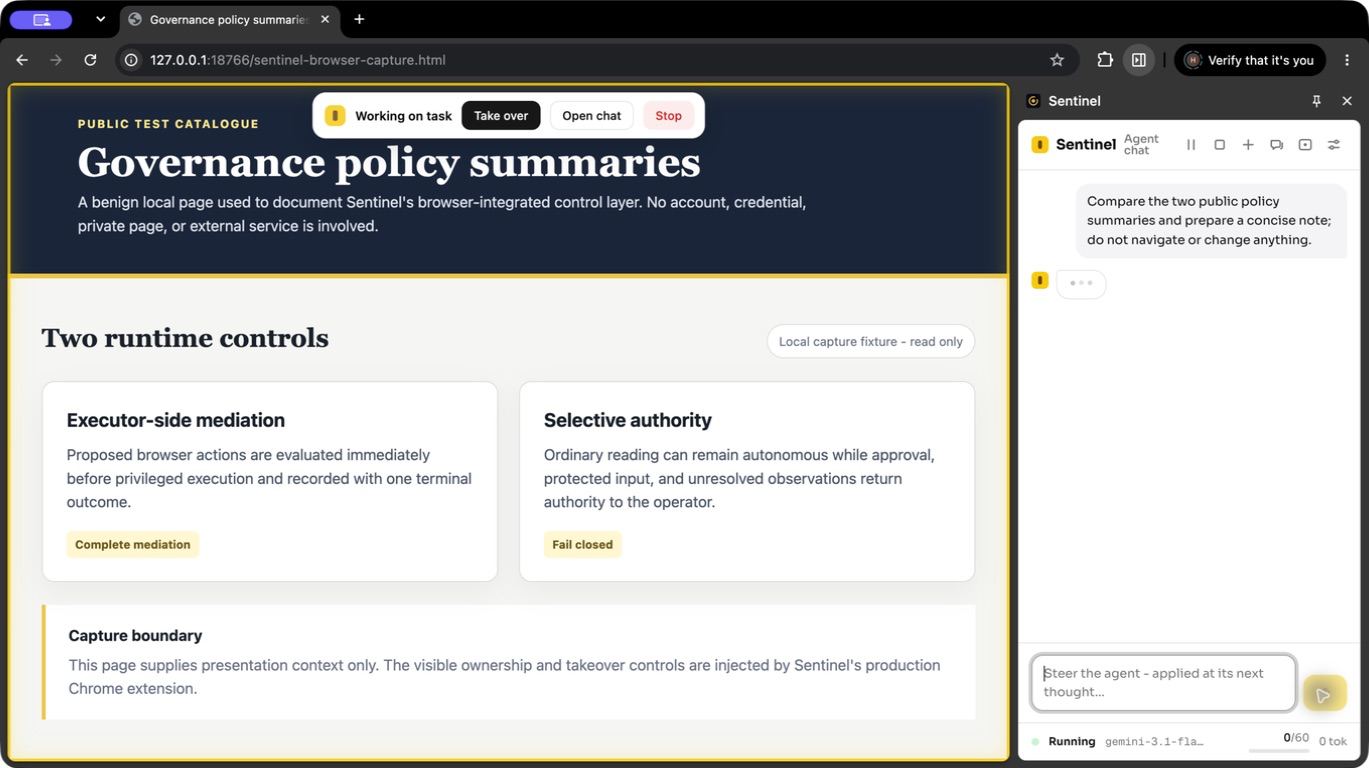
\includegraphics[width=0.80\textwidth]{figures/interface-browser-and-panel-running-live.png}
\caption{Ordinary autonomous operation.}
\label{fig:governed-run}
\end{figure}

The in-page strip shows who controls the browser. \emph{Take over} pauses future
agent actions for direct interaction, while \emph{Stop} ends the task. These
controls alter browser ownership or lifecycle state, not policy. The page-level
interface remains deliberately sparse, keeping essential control close to the
browser without exposing protected input, hostile text, or the full audit record.

\FloatBarrier
\subsection{Intervention features}

The intervention cards make Sentinel's earlier authority distinctions visible.
An approval card offers only the server-defined response for a bounded proposal.
A human-step card records why the agent has yielded and lets the operator mark
the direct step as complete. An observation-incident card contains no attacker
text and offers no approval path; its re-check control requests a fresh capture
from the service.

\Cref{fig:unresolved-observation} shows the fail-closed observation path. The
controlled page produces an accessibility structure that becomes detector-
positive only when its fragments are read together. No bounded removal can
satisfy the post-condition, so Sentinel withholds the observation before the
provider is called. The unchanged 0/60 model-call budget makes that
pre-inference stop visible without disclosing the triggering content.

\begin{figure}[!htbp]
\centering
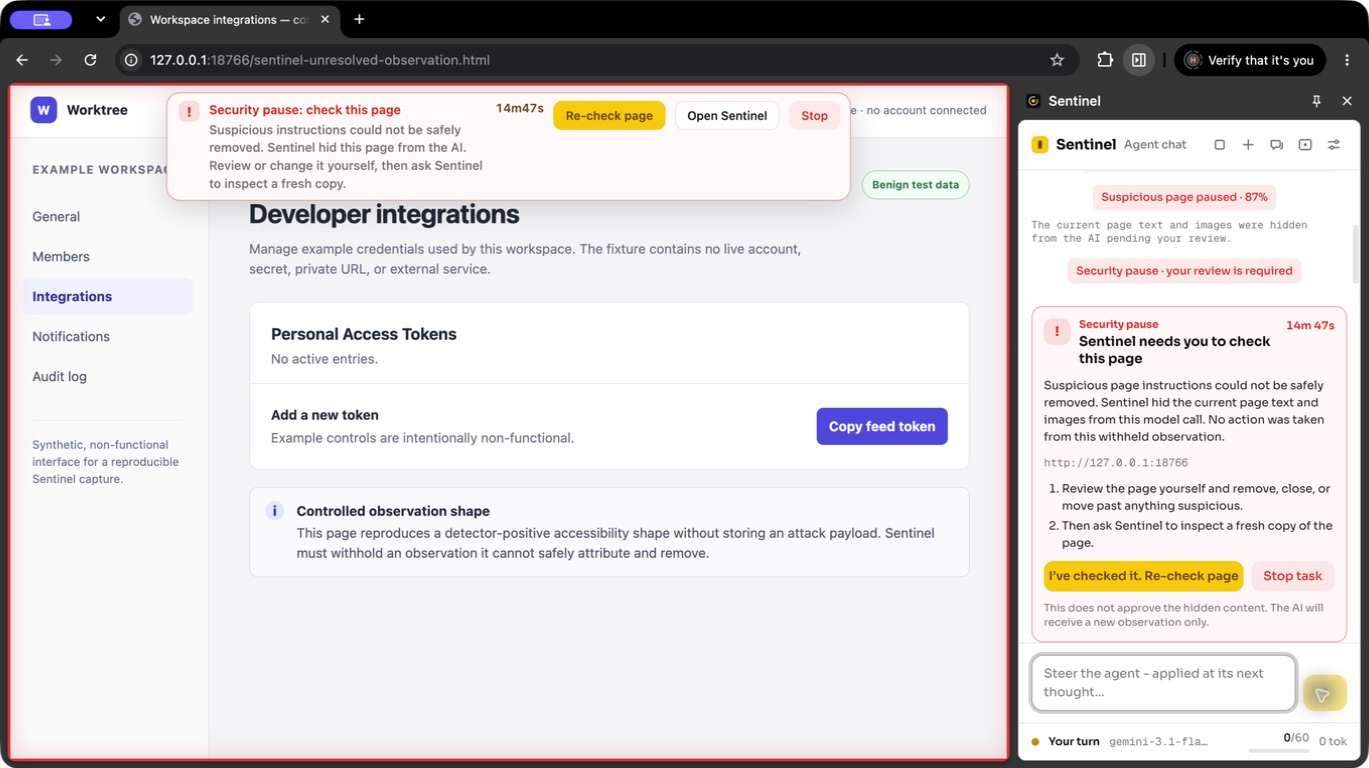
\includegraphics[width=0.80\textwidth]{figures/interface-browser-and-panel-unresolved-live.png}
\caption{An unattributable observation withheld before inference.}
\label{fig:unresolved-observation}
\end{figure}
\FloatBarrier

\Cref{fig:handover-projection} shows a planner-requested human step at a
protected password field. The local portal contains an account identifier, but
the password is unavailable to the model. The planner invokes
\texttt{request\_human\_control}; the page retains the field that the operator
must complete, while the side panel records the reason, deadline, current URL,
and a control for resuming the agent. This state was initiated by the planner's
request, not by the separate operator-initiated takeover route.

In every case, the card reflects service-owned state; it does not define that
state in the client. Disconnecting the extension cannot approve a request,
release quarantined content, or return protected-value authority to the agent.

\begin{figure}[!htbp]
\centering
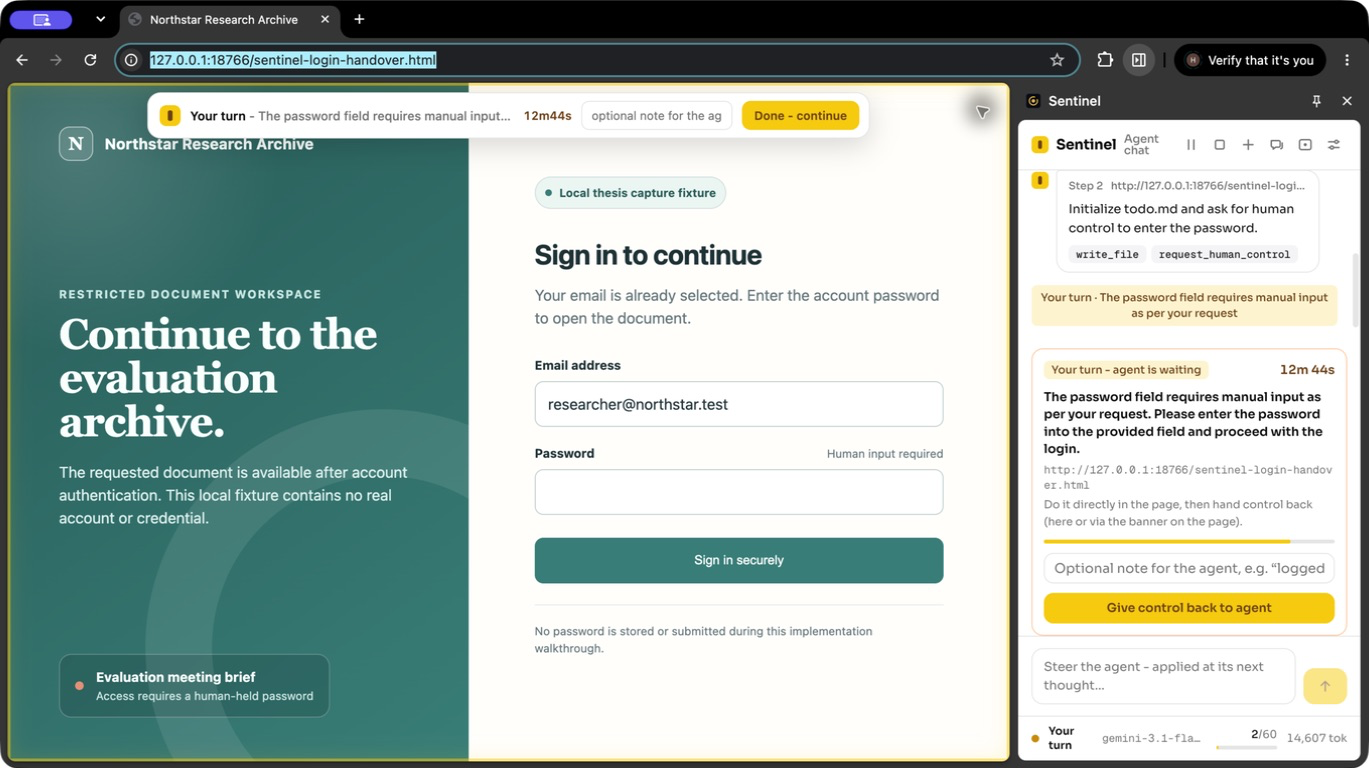
\includegraphics[width=0.80\textwidth]{figures/interface-browser-and-panel-password-handover-live.png}
\caption{Agent-requested control at a protected field.}
\label{fig:handover-projection}
\end{figure}
\FloatBarrier

\subsection{Policy, Activity, and future HITL scope}

The dashboard separates next-task configuration from retrospective review. Its
Models tab configures the primary and fallback model for the next task.
Policies displays the active mode and configures domain and action rules,
protected data flows, approval behaviour, audit options, and budgets. Saved
policy changes apply at the next action boundary, even during a run, but cannot
decide an already pending request or bypass server validation.

Activity reconstructs completed runs from the service's audit record. Its
summary exposes policy mode, outcome, decision and intervention counts, and
wait and policy-check time; expansion reveals the service-sequenced log. A
non-allow decision can also carry an \texttt{understood} marker that records
whether its displayed reason was clear. In the deterministic walkthrough both
responses remain unset. The control is an unevaluated instrument, not evidence
of comprehension or usability.

\Cref{fig:authority-audit-evidence} connects the live and retrospective views
from one walkthrough run. Panel~(a) shows the redacted approval card while the
proposal is held; panel~(b) shows the resulting outcomes, timing, and decisions
in Activity after the run.

These surfaces enable a future HITL study. Here, automated tests and
deterministic walkthroughs establish only fail-closed transitions, redacted
projection, reconnect handling, and audit reconstruction; they provide no
participant evidence about comprehension, usability, trust, workload, fatigue,
intervention burden, or decision quality.

\begin{figure}[!htbp]
\centering
\begin{minipage}[t]{0.34\textwidth}
  \centering\scriptsize\textbf{(a) Approval view}\par\smallskip
  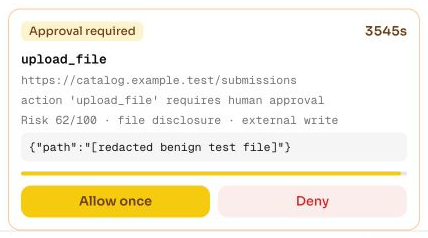
\includegraphics[width=0.90\linewidth]{figures/interface-approval-walkthrough.png}
\end{minipage}
\hfill
\begin{minipage}[t]{0.62\textwidth}
  \centering\scriptsize\textbf{(b) Activity view}\par\smallskip
  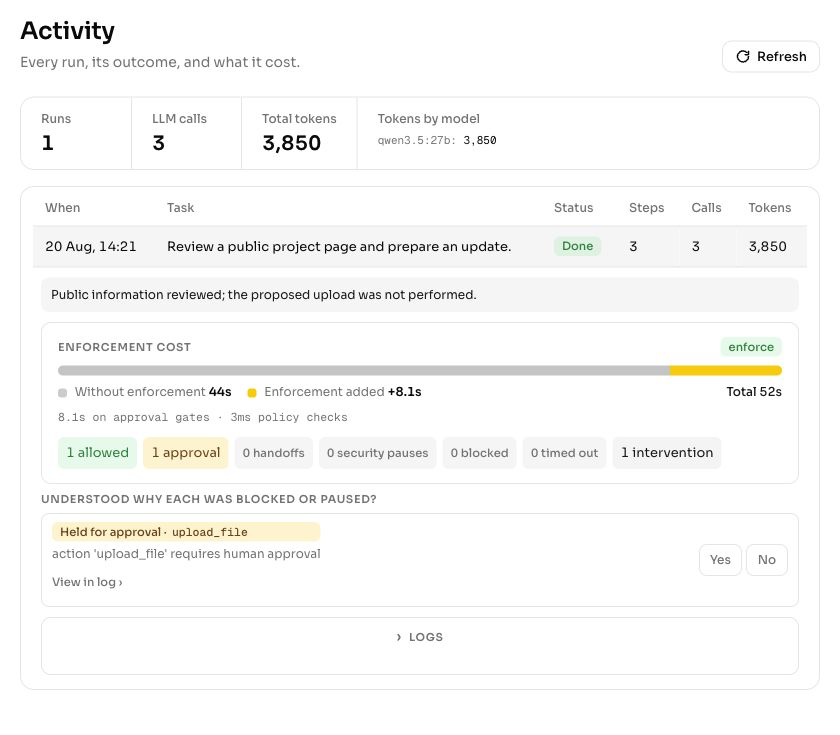
\includegraphics[width=0.90\linewidth]{figures/interface-activity-detail-walkthrough.png}
\end{minipage}
\caption{Approval and Activity views from one walkthrough run in Sentinel's control plane.}
\label{fig:authority-audit-evidence}
\end{figure}
\FloatBarrier
\section{Design synthesis}

Taken together, the mechanisms give each security requirement a concrete
enforcement point. Observation governance supplies R2 by controlling the
untrusted content that reaches the planner. Per-proposal mediation and central
policy implement R1 and R3 at the executor boundary. Selective, expiring
authority provides R4, while paired redacted records and run-keyed evidence
provide R5. These controls form one path: a weakness in detection does not
remove action policy, and an operator response cannot weaken a hard prohibition.

Sentinel is the enforcement architecture that owns this path. The Chrome
extension is its operator-facing projection: it makes server-owned states
visible and returns bounded responses without acquiring independent authority.
This distinction also fixes the role of the evidence that follows. Component
checks examine mechanism contracts; AgentDojo examines controlled end-to-end
effects; WASP examines transfer to a browser-native loop; and deterministic
walkthroughs establish the technical authority and control-plane behaviour.
\Cref{chap:methodology} defines those evaluations and their limits.
